\chapter{Results}
\section{Motion Segmentation}
We were able to achieve data transmission from the robot with very
less latency. We also demonstrated the use of gestures in the virtual
reality platform to alter the robot's navigation parameters. A sample
video showing this can be found \href{https://vimeo.com/192891505}{\bf
  HERE}. Using Mozilla as the platform for visualization of data allows implementation of MozVR based APIs in the system. The VR system was able to understand gestures (left swipe, right swipe, and pinch) using the installed infra-red optical trackers.
\begin{figure}[h!]
  \begin{center}
    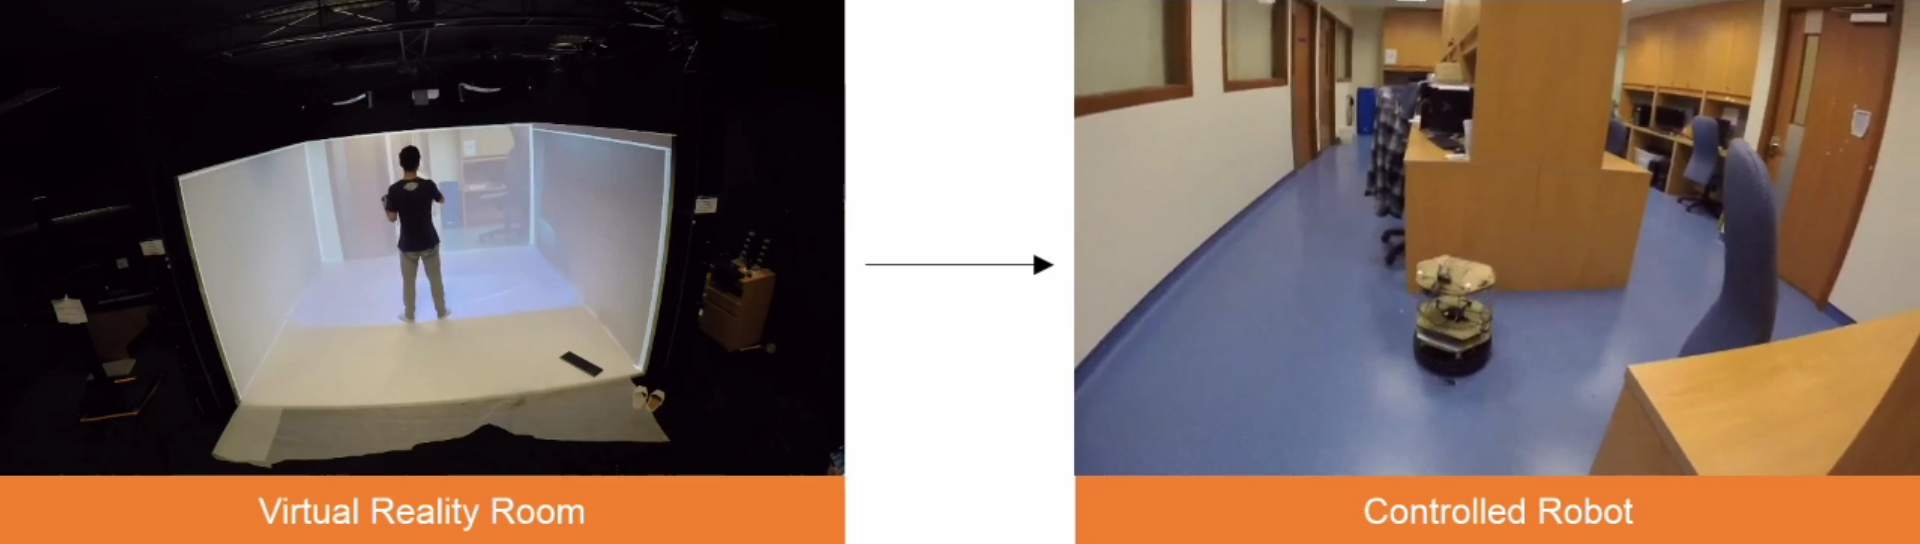
\includegraphics[width=0.99\textwidth]{figures/motion-seg/result}% This is a *.jpg file
  \end{center}
  \caption{Real-Time Robot Control And Data Visualization.}
  \label{fig:result-motion}
\end{figure}

\section{Vibro-Tactile Haptic Glove}
The first, second and third generation of the vibro-tactile haptic
glove use amplitude modulation to control the vibration intensity of
each actuator. For the first generation of haptic glove, we conducted
an experiment where random tactile stimulus was tested by blindfolding
and asking the user the site of perception. The haptic gloves
demonstrated the capability of rendering spatial touch information to
users. The perception results for 30 participants are shown in
Fig\ref{fig:glove-active}. Since the third generation of haptic glove
is built on same design principle, we expect similar results.

\begin{figure}[!ht]
  \centering
  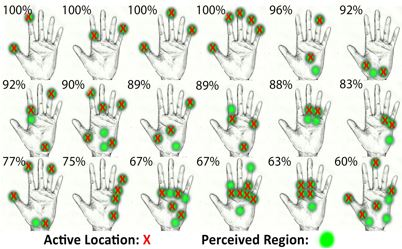
\includegraphics[width=10cm]{figures/figure6.jpg}
  \caption{Perception of active region.}
  \label{fig:glove-active}
\end{figure}


\section{Virtual Reality Room}

Though Marker based gesture recognition has received some level of
criticisms. The marker tracking systems still have various advantages
that cannot be replaced by other computer vision methods. In this
period of work we used the {\bf flystick}(Fig\ref{fig:flystick}) to
test the pick and place system:
\begin{figure}[!ht]
  \centering
  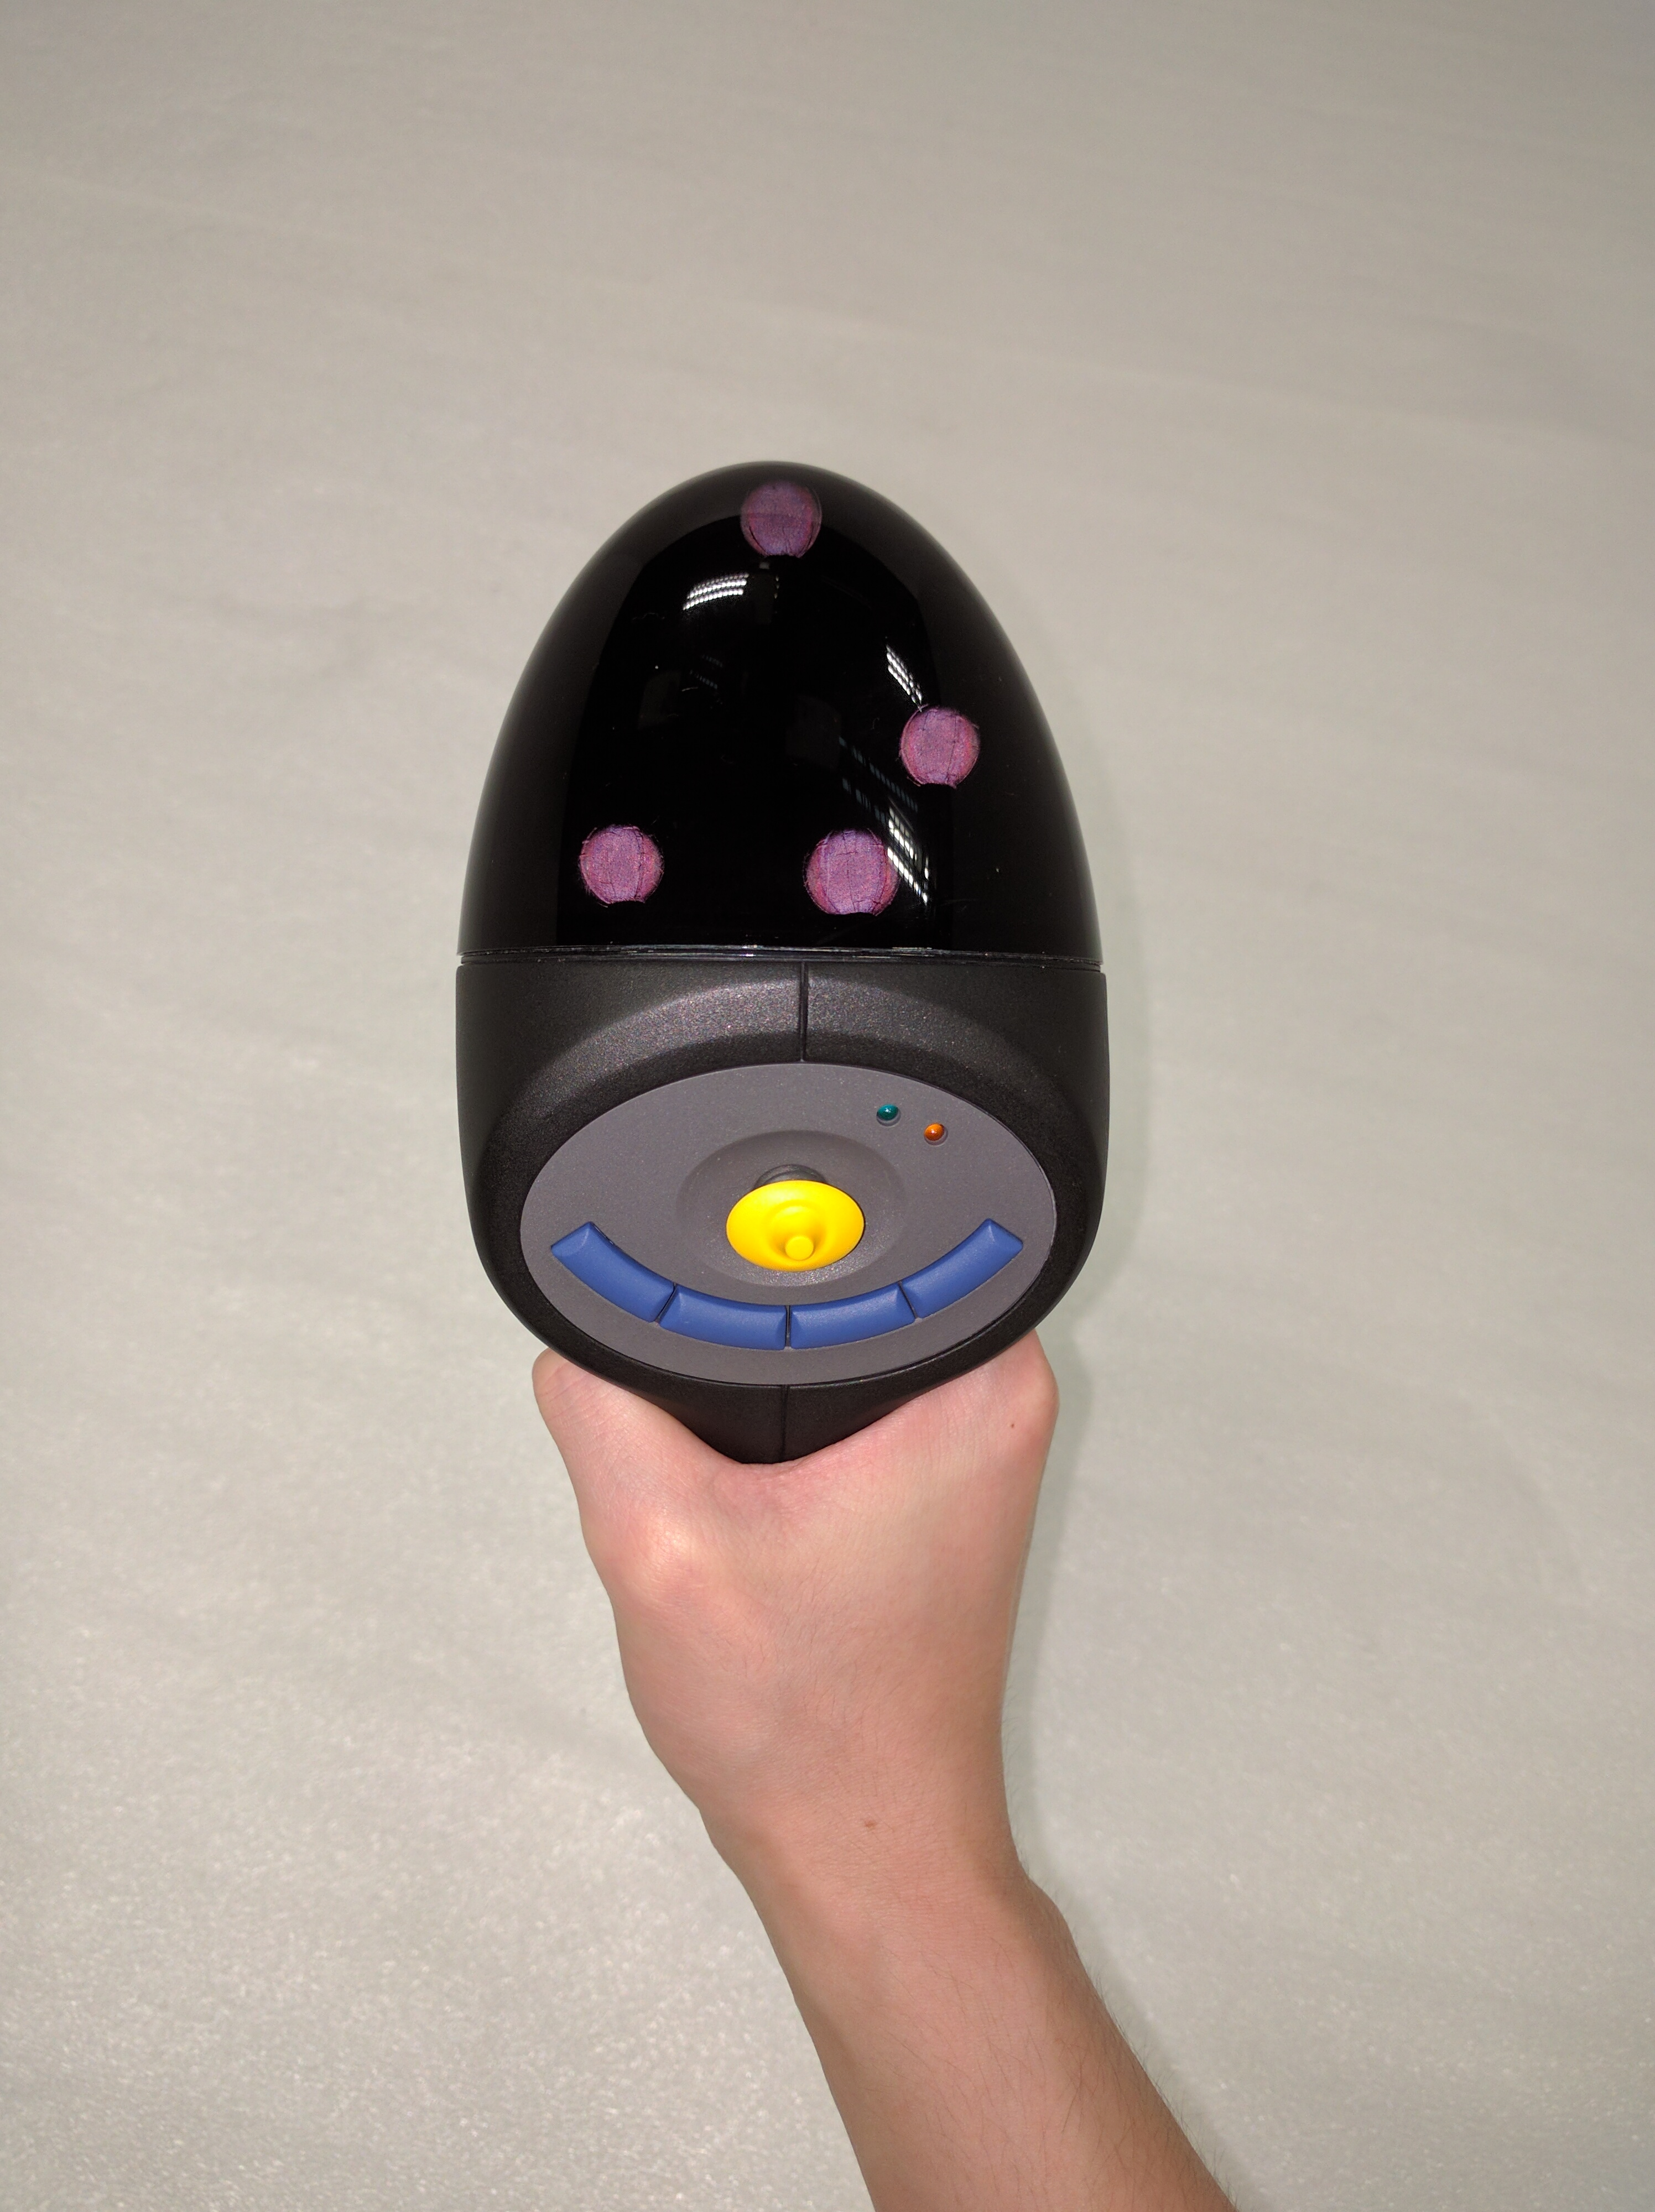
\includegraphics[width=8cm]{figures/flystick.jpg}
  \caption{CAVE Flystick}
  \label{fig:flystick}
\end{figure}

The flystick provides 5 buttons and an axis, which satisfies both
scenarios in our experiment.

For the further development of the system. We collected data with
20 markers randomly put on a user's arms and
chest. Fig\ref{fig:markers} shows a data frame where the user stands
in the CAVE VR room:

\begin{figure}[!ht]
  \centering
  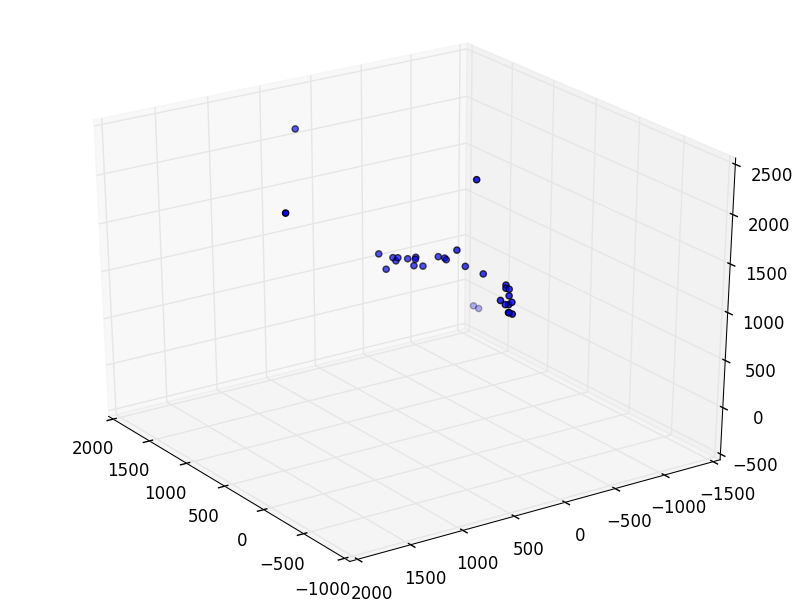
\includegraphics[width=8cm]{figures/markers.png}
  \caption{Visualization of Markers on a User's Body}
  \label{fig:markers}
\end{figure}



%%% Local Variables:
%%% mode: latex
%%% TeX-master: "../master"
%%% End:
